\documentclass[tikz,border=5pt]{standalone}

\usepackage{fontspec}
\setmainfont{Libertinus Serif}

\usepackage{tikz}
\usetikzlibrary{calc,angles,quotes}

\begin{document}

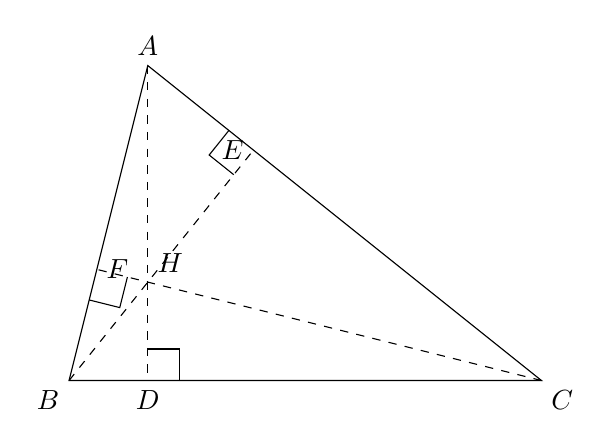
\begin{tikzpicture}[scale=2]

% Triangle vertices
\coordinate (A) at (0.5,2);
\coordinate (B) at (0,0);
\coordinate (C) at (3,0);

% Draw triangle
\draw (A) -- (B) -- (C) -- cycle;

% Feet of perpendiculars using projection
\coordinate (D) at ($(B)!(A)!(C)$);
\coordinate (E) at ($(C)!(B)!(A)$);
\coordinate (F) at ($(A)!(C)!(B)$);

% Orthocenter (intersection of altitudes)
% constructed as intersection of two altitudes
\coordinate (H) at (intersection of A--D and B--E);

% Altitudes
\draw[dashed] (A) -- (D);
\draw[dashed] (B) -- (E);
\draw[dashed] (C) -- (F);

% Right angle marks using proper geometry
\pic[draw, angle radius=4mm] {right angle = A--D--C};
\pic[draw, angle radius=4mm] {right angle = B--E--A};
\pic[draw, angle radius=4mm] {right angle = C--F--B};

% Labels
\node[above] at (A) {$A$};
\node[below left] at (B) {$B$};
\node[below right] at (C) {$C$};

\node[below] at (D) {$D$};
\node[left] at (E) {$E$};
\node[right] at (F) {$F$};

\node[above right] at (H) {$H$};

\end{tikzpicture}

\end{document}
